\section{Akvizicija zvuka}
\label{sec:acq}

Podsustav za akviziciju zvuka je usko vezan uz računalnu platformu na kojoj
je sustav implementiran jer izravno komuninicira
sa sustavom koji prikuplja stvarne signale sa senzora (mikrofona).
Kao platforma za implementaciju opisanog sustava odabran je razvojni sustav ESP32 Lyrat Development Board \cite{lyrat} koji ima već ugrađen mikrofon i audio kodek
s kojim je moguće komunicirati putem I2S protokola. Na slici
\ref{pic:esp} prikazan je blok dijagram ESP32 razvojne platforme.

\begin{figure}[htb]
    \centering
    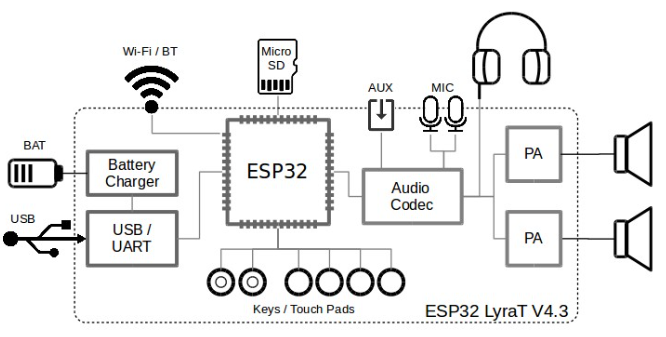
\includegraphics[width=0.75\linewidth]{Chapters/struktura_sustava/akvizicija/lyrat.png} 
    \caption{ESP32 Lyrat \cite{lyrat}}
    \label{pic:esp}
\end{figure}

Najvažniji dio razvojne platforme je ESP32-WROVER-E mikrokontroler
na kojem je implementirano cjelokupno programsko rješenje za prepoznavanje govornih naredbi. Upravo on je taj mikrokontroler zadužen za komunikaciju s ES8388 
audio kodekom \cite{es8388}. ES8388 je integrirani sklop koji na spomenutoj
platformi služi za analogno-digitalnu (engl. \textit{ADC}) te digitalno-analognu 
(engl. \textit{DAC}) pretvorbu, tj. upravljanje audio ulazom (mikrofon) te audio
izlazom (AUX priključak). Mikrokontroler putem I2C sučelja konfigurira kodek,
dok zvučne signale prikuplja s mikrofona putem I2S sučelja. Budući da je ESP32 Lyrat
platforma prilagođena razvoju audio sustava, konfiguracija i puštanje u pogon
akvizicije zvuka je vrlo jednostavno. U programskom kodu \ref{code:ES8388init}
prikazana je inicijalizacija kodeka.

\begin{lstlisting}[language=C++, caption=Inicijalizacija kodeka, label=code:ES8388init]
    audio_board_handle_t board_handle = audio_board_init();
    audio_hal_ctrl_codec(board_handle->audio_hal, AUDIO_HAL_CODEC_MODE_ENCODE, AUDIO_HAL_CTRL_START);
\end{lstlisting}

Sav posao koji se nalazi iza prikazanih naredbi obavlja ESP-ADF
(engl. \textit{Espressif Audio Development Framework}). To je biblioteka koja pojednostavljuje
razvoj aplikacija vezanih za obradu zvuka i osnovne zadatke, kao što su akvizicija, kodiranje i 
dekodiranje različitih formata audio zapisa te komunikacija s računalom ili 
memorijskom karticom.
Nakon inicijalizacije kodeka i definiranja konfiguracije postavki I2S komunikacije,
potrebno je pokrenuti protočni akvizicijski sustav (engl. \textit{pipeline}), 
a to je prikazano u programskom kodu \ref{code:pipeline} .

\begin{lstlisting}[language=C++, caption=Pokretanje akvizicijskog sustava, label=code:pipeline]
    ESP_LOGI(TAG, "Creating i2s stream");
    audio_element_handle_t i2s_stream_reader;
    i2s_stream_cfg_t i2s_cfg = I2S_STREAM_CFG_DEFAULT();
    i2s_cfg.type = AUDIO_STREAM_READER;
    i2s_cfg.i2s_port = I2S_NUM_0;
    i2s_cfg.i2s_config = i2s;
    i2s_stream_reader = i2s_stream_init(&i2s_cfg);

    ESP_LOGI(TAG, "Creating audio pipeline");
    audio_pipeline_handle_t pipeline;
    audio_pipeline_cfg_t pipeline_cfg = DEFAULT_AUDIO_PIPELINE_CONFIG();
    pipeline = audio_pipeline_init(&pipeline_cfg);
    audio_pipeline_register(pipeline, i2s_stream_reader, "i2s");
    audio_pipeline_run(pipeline);
\end{lstlisting}

Frekvencija otipkavanja postavljena u konfiguraciji iznosi 16000 Hz što
je dovoljno za ovakav tip sustava za prepoznavanje glasovnih naredbi \cite{wardentinyml}.
Nakon pokretanja akvizicijskog podsustava preostalo je uzimati nove
podatke s kraja protočne strukture podsustava. Konstantno uzimanje novih uzoraka, tj. komunikacija
s ES8388 kodekom, odvojeno je u posebnu dretvu. Na taj način programski je 
odvojena akvizicija sirovih uzoraka zvuka od ostatka sustava u kojima se obavlja obrada nad njima. Ovaj podsustav je proizvođač novih podataka, dok je ostatak sustava potrošač, koji je također realiziran u posebnoj dretvi. Kako su prikupljanje podataka i njihova obrada realizirani pomoći dvije odvojene dretve, potrebno je implementirati pouzdan i efikasan način komunikacije između njih. Za tu svrhu odabran je
kružni međuspremnik (engl. \textit{ring buffer}) koji omogućuje asinkrono pisanje i čitanje. Implementacija takve strukture dostupna je kao objekta FreeRTOS-a 
\cite{ringbufferrr}, koji je odabran kao operacijski sustav za rad u stvarnom vremenu na kojem je realizirano višedretveno rješenje. 


\begin{lstlisting}[language=C++, caption=Razred AudioRecorder, label=code:AudioRecorder]
class AudioRecorder
{
    private:
        uint32_t sampleRate;
        RingbufHandle_t ringBuffer;
        TaskHandle_t captureAudioHandle;
        static void captureAudioTask(void* pvParameters);
    public:
        AudioRecorder(uint32_t sampleRate) : sampleRate(sampleRate), 
                                             ringBuffer(NULL), 
                                             captureAudioHandle(NULL) {}
        uint32_t getSamples(int16_t* samples, size_t numOfSamples);
};
\end{lstlisting}

Opisani podsustav za akviziciju zvuka u programskom kodu strukturiran je u razred imena 
AudioRecorder \ref{code:AudioRecorder} kako bi ga se lakše koristilo. Razred sadrži metodu
\texttt{uint32\_t getSamples(int16\_t* samples, size\_t numOfSamples)} koja 
omogućuje dohvaćanje proizvoljnog broja \texttt{uint16\_t} podataka jer 
se akvizirani zvučni signal pohranjuje u tom obliku. U glavnoj petlji sustava potrebno je kreirati objekt
razreda AudioRecorder, alocirati memorijski spremnik za dohvaćanje podataka i kontinuirano
pozivati navedenu funkciju koja kao argumente prima pokazivač na alocirani spremnik
i željeni broj audio uzoraka za dohvat.

Spomenuta modularnost ostvarena je tako što je funkcionalnost prikupljanja
novih zvučnih uzoraka sadržana u opisanom razredu. Pokretanje cjelokupnog sustava
na drugoj platformi koja ima drugi audio kodek, drugačiji mikrofon ili se 
radi o drugom mikrokontroleru, bit će moguće implementiranjem novog razreda koji
podržava zadano drugačije sučelje.